\documentclass[9pt]{beamer}
% package list
\usepackage{./Amsterdam}
\usepackage{graphicx}
\usepackage{wrapfig}
% setting 
\definecolor{MidnightBlue}{RGB}{0,103,149}
\setbeamertemplate{frametitle}{\hspace{-0.5cm}\bf\insertframetitle}
% prensentation info
\title[Application of Conditional Random Field in Image Salient Object Detection]
{\bf Application of Conditional Random Field in \\Image Salient Object Detection with \\Local, Regional, Global Feature Extraction}
\author[Jimmy Lin and Chris Claoue Long]{\bf Jimmy Lin \\Chris Claoue Long}
\institute{\bf Dr. Stephen Gould\\[0.3cm] College of Engineering and Computer Science \\Australian National University}
\date{\bf \today}
% new command definition
\DeclareMathOperator*{\argmin}{arg\,min}
\DeclareMathOperator*{\argmax}{arg\,max}
%%% beginning of document
\begin{document}
\begin{large}
\frame{\titlepage }
\end{large}

%{{{ Introduction
\section{Introduction}
\frame{
    \frametitle{Introduction}
}
%}}}

%{{{ Related Works
\section{Related Works}
\frame{
    \frametitle{Related Works}
}
%}}}

%{{{ Problem Formulation
\section{Problem Formulation}
\frame{
    \frametitle{Formulation}
}
%}}}

%{{{ Feature Extraction
\section{Feature Extraction}
\frame{
    \newcommand{\imageVSpacing}{\vspace*{0.5cm}}
    {\bf \sectionpage}
    \begin{center}
    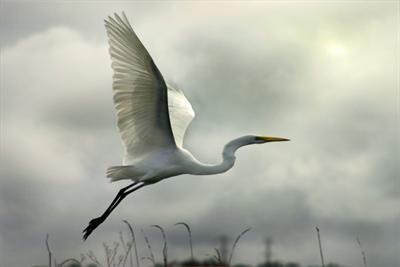
\includegraphics[width=0.72in,height=0.52in]{./MC_image/1.jpg}
    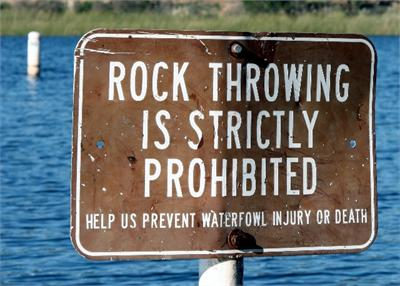
\includegraphics[width=0.72in,height=0.52in]{./MC_image/2.jpg}
    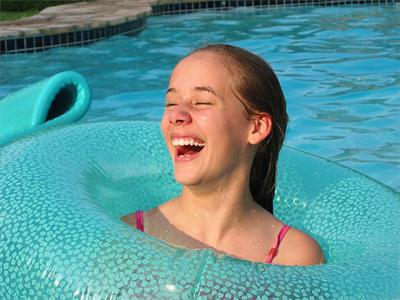
\includegraphics[width=0.72in,height=0.52in]{./MC_image/3.jpg} 
    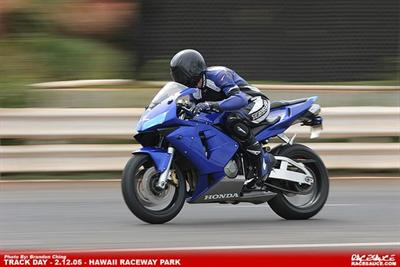
\includegraphics[width=0.72in,height=0.52in]{./MC_image/4.jpg} 
    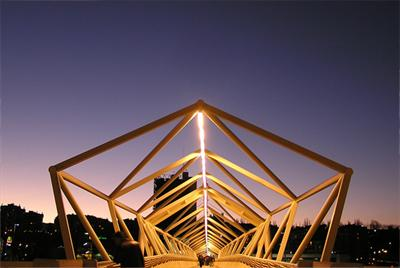
\includegraphics[width=0.72in,height=0.52in]{./MC_image/5.jpg} 
    \\
    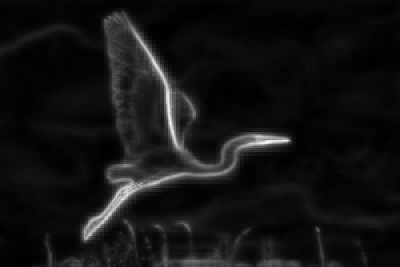
\includegraphics[width=0.72in,height=0.52in]{./MC_image/1_MC.jpg}
    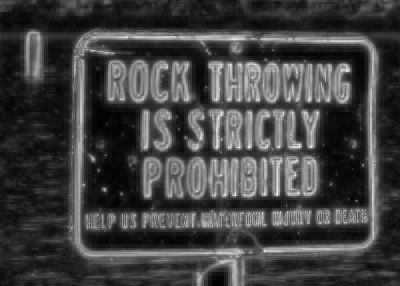
\includegraphics[width=0.72in,height=0.52in]{./MC_image/2_MC.jpg}
    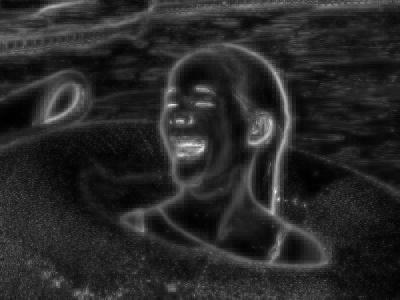
\includegraphics[width=0.72in,height=0.52in]{./MC_image/3_MC.jpg}
    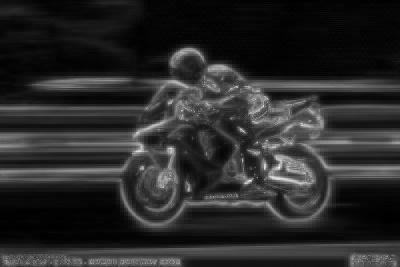
\includegraphics[width=0.72in,height=0.52in]{./MC_image/4_MC.jpg}
    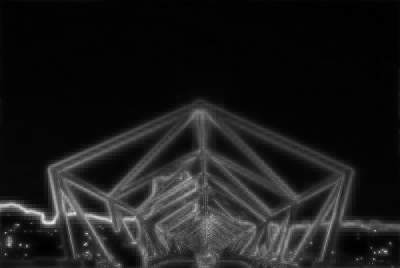
\includegraphics[width=0.72in,height=0.52in]{./MC_image/5_MC.jpg}
    \\
    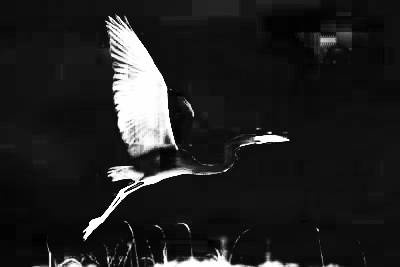
\includegraphics[width=0.72in,height=0.52in]{./MC_image/1_CSD.jpg}
    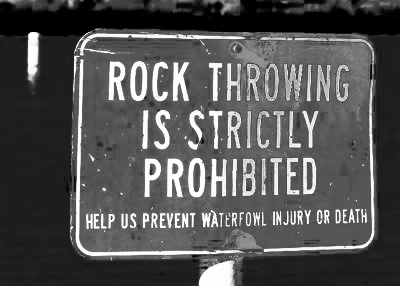
\includegraphics[width=0.72in,height=0.52in]{./MC_image/2_CSD.jpg}
    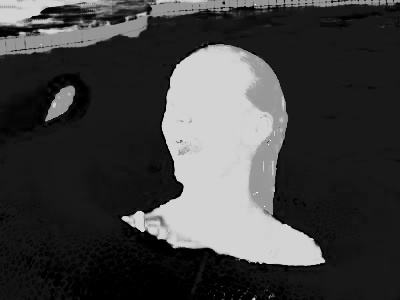
\includegraphics[width=0.72in,height=0.52in]{./MC_image/3_CSD.jpg}
    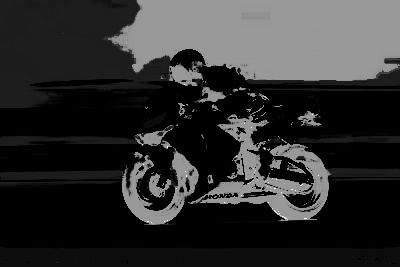
\includegraphics[width=0.72in,height=0.52in]{./MC_image/4_CSD.jpg}
    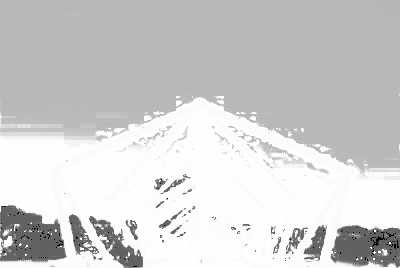
\includegraphics[width=0.72in,height=0.52in]{./MC_image/5_CSD.jpg}
\end{center}
}
\frame{
    \frametitle{Local: Multiscale Contrast}
}

\frame{
    \frametitle{Regional: Center-Surround Histogram}

}
\frame{
    \frametitle{Global: Color Spatial Distribution}
    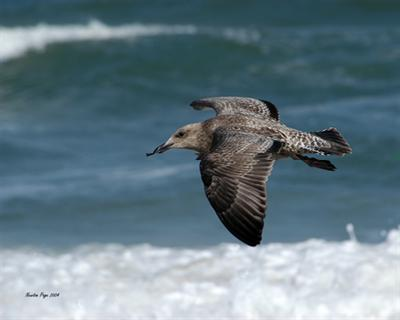
\includegraphics[width=0.72in,height=0.52in]{./CSD_image/1.jpg}
    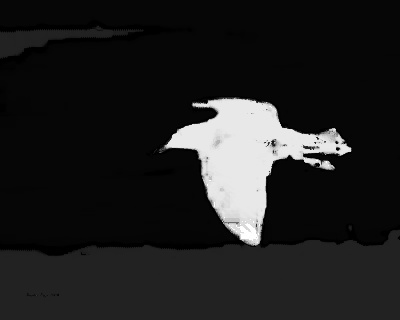
\includegraphics[width=0.72in,height=0.52in]{./CSD_image/1_CSD.jpg}
    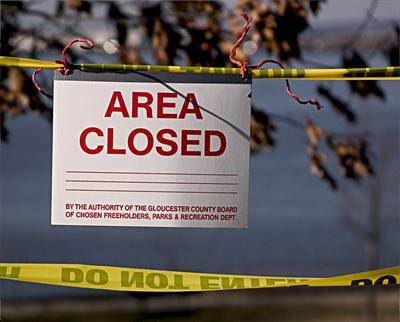
\includegraphics[width=0.72in,height=0.52in]{./CSD_image/2.jpg}
    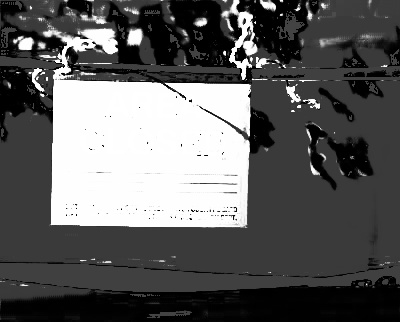
\includegraphics[width=0.72in,height=0.52in]{./CSD_image/2_CSD.jpg}
    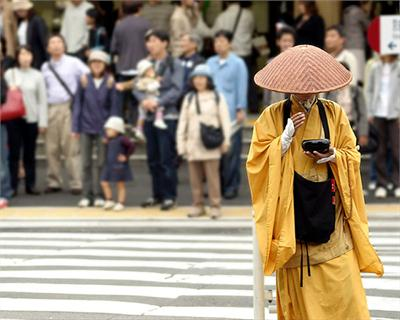
\includegraphics[width=0.72in,height=0.52in]{./CSD_image/3.jpg}
    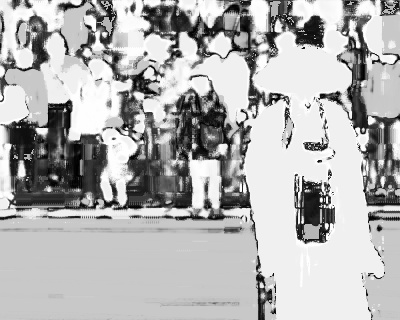
\includegraphics[width=0.72in,height=0.52in]{./CSD_image/3_CSD.jpg}
}
%}}}

%{{{ CRF content
\section{Conditional Random Field}
\frame{
    \frametitle{Learning}
}
\frame{
    \frametitle{Inference}
}
%}}}

%{{{ Reference
\section{Reference}
\frame{
    \frametitle{Reference}
    \begin{thebibliography}{9}
        \bibitem{ConcreteMath} Liu, Tie, et al. "Learning to detect a salient object."\textit{ Computer Vision and Pattern Recognition, 2007. CVPR'07. IEEE Conference on. IEEE, 2007. }
        \bibitem{ConcreteMath} Liu, Tie, et al. "Learning to detect a salient object."\textit{ Pattern Analysis and Machine Intelligence, IEEE Transactions on 33.2 (2011): 353-367.}
        \bibitem{ConcreteMath} Itti, Laurent, Christof Koch, and Ernst Niebur. "A model of saliency-based visual attention for rapid scene analysis."\textit{ Pattern Analysis and Machine Intelligence, IEEE Transactions on 20.11 (1998): 1254-1259.}
        \bibitem{ConcreteMath} Ma, Yu-Fei, and Hong-Jiang Zhang. "Contrast-based image attention analysis by using fuzzy growing."\textit{ Proceedings of the eleventh ACM international conference on Multimedia. ACM, 2003.} 
        \bibitem{ConcreteMath} Stephen Gould, "DARWIN: A Framework for Machine Learning and Computer Vision Research and Development", \textit{Journal of Machine Learning Research (JMLR), 13(Dec):3533−3537, 2012}.
    \end{thebibliography}
}
%}}}
\end{document}
